%  article.tex (Version 3.3, released 19 January 2008)
%  Article to demonstrate format for SPIE Proceedings
%  Special instructions are included in this file after the
%  symbol %>>>>
%  Numerous commands are commented out, but included to show how
%  to effect various options, e.g., to print page numbers, etc.
%  This LaTeX source file is composed for LaTeX2e.

%  The following commands have been added in the SPIE class 
%  file (spie.cls) and will not be understood in other classes:
%  \supit{}, \authorinfo{}, \skiplinehalf, \keywords{}
%  The bibliography style file is called spiebib.bst, 
%  which replaces the standard style unstr.bst.  

\documentclass[]{spie}  %>>> use for US letter paper
%%\documentclass[a4paper]{spie}  %>>> use this instead for A4 paper
%%\documentclass[nocompress]{spie}  %>>> to avoid compression of citations
%% \addtolength{\voffset}{9mm}   %>>> moves text field down
%% \renewcommand{\baselinestretch}{1.65}   %>>> 1.65 for double spacing, 1.25 for 1.5 spacing 
%  The following command loads a graphics package to include images 
%  in the document. It may be necessary to specify a DVI driver option,
%  e.g., [dvips], but that may be inappropriate for some LaTeX 
%  installations. 
\usepackage[]{graphicx}
\usepackage{amsmath}

\title{Longitudinal assessment of treatment effects on pulmonary ventilation using 1H/3He MRI multivariate templates} 

%>>>> The author is responsible for formatting the 
%  author list and their institutions.  Use  \skiplinehalf 
%  to separate author list from addresses and between each address.
%  The correspondence between each author and his/her address
%  can be indicated with a superscript in italics, 
%  which is easily obtained with \supit{}.

\author{Nicholas J. Tustison\supit{a}, Benjamin Contrella\supit{a}, Talissa A. Altes\supit{a}, Brian B. Avants\supit{b}, Eduard E. de Lange\supit{a}, John P. Mugler III\supit{a}
\skiplinehalf
\supit{a}Dept. of Radiology and Medical Imaging, Univ. of Virginia, Charlottesville, Virginia, USA\\
\supit{b}PICSL, Univ. of Pennsylvania, Philadelphia, Pennsylvania, USA
}

%>>>> Further information about the authors, other than their 
%  institution and addresses, should be included as a footnote, 
%  which is facilitated by the \authorinfo{} command.

\authorinfo{Further author information: (Send correspondence to N.J.T.)\\
            N.J.T.: E-mail: njt4n@virginia.edu, Telephone: 1 434 924 7730}
%%>>>> when using amstex, you need to use @@ instead of @
 

%%%%%%%%%%%%%%%%%%%%%%%%%%%%%%%%%%%%%%%%%%%%%%%%%%%%%%%%%%%%% 
%>>>> uncomment following for page numbers
% \pagestyle{plain}    
%>>>> uncomment following to start page numbering at 301 
%\setcounter{page}{301} 
 
  \begin{document} 
  \maketitle 

%%%%%%%%%%%%%%%%%%%%%%%%%%%%%%%%%%%%%%%%%%%%%%%%%%%%%%%%%%%%% 
\begin{abstract}

The utility of pulmonary functional imaging techniques, such as
hyperpolarized 3He MRI, has encouraged their inclusion in research
studies for longitudinal assessment of disease progression and the study of 
treatment effects.  We present methodology for performing voxelwise
statistical analysis of ventilation maps derived from 
hyperpolarized 3He MRI which incorporates multivariate template
construction using simultaneous acquisition of 1H and
3He images.  Additional processing steps include intensity normalization,
bias correction,
4-D longitudinal segmentation, and generation of expected ventilation
maps prior to voxelwise regression analysis.  Analysis is demonstrated 
on a cohort of eight individuals with diagnosed cystic fibrosis (CF) 
undergoing treatment imaged five times every two weeks with a prescribed
treatment schedule.
\end{abstract}

\keywords{hyperpolarized 3He, pulmonary segmentation, regression analysis, ventilation defects}

%%%%%%%%%%%%%%%%%%%%%%%%%%%%%%%%%%%%%%%%%%%%%%%%%%%%%%%%%%%%%
\section{INTRODUCTION}
\label{sec:intro}  % \label{} allows reference to this section

Due to the heterogeneous nature of pathologic lung processes, studies of progression and treatment are complex and best assessed through integrated longitudinal studies.  Many of the longitudinal pulmonary studies to date have used 
spirometry to evaluate lung function although imaging is rapidly being adopted given its increased
spatial sensitivity.  Over the past decade, hyperpolarized 3He gas has been successfully used to visualize ventilation defects in the lungs\cite{lange1999} with significant potential for computational analysis.\cite{tustison2011}  
Given the nature of longitudinal studies in which a single subject is imaged numerous times, we detail
a framework for aligning the subject's individual time point images to a common subject-specific 
reference space in preparation for
voxelwise statistical regression.  This, in turn, produces treatment effect maps which simultaneously condenses the amount of longitudinal information while retaining the spatial sensitivity of imaging.  These processes are illustrated with a cohort of eight individuals diagnosed with CF imaged every two weeks (five total time points) over the course of experimental treatment.  The scope of this work is limited to methodological description with detailed clinical hypotheses and findings reported elsewhere.\cite{altes2012}.


%%%%%%%%%%%%%%%%%%%%%%%%%%%%%%%%%%%%%%%%%%%%%%%%%%%%%%%%%%%%%
\section{MATERIALS AND METHODS} 


\subsection{Image Analysis}

In our earlier work\cite{tustison2011}, we described a ventilation-based segmentation workflow applied to single time point 3He data and provided evidence of its excellent performance relative to trained human readers.  In contrast, this work is concerned with the additional complexity of tracking relative longitudinal changes over multiple image acquisitions within a single subject.   As a general overview, analysis of longitudinal data comprises the following basic steps:
\begin{itemize}
\item multimodal atlas construction for each subject (cf Fig. \ref{fig:template}), 
\item intensity normalization\cite{nyul2000} and bias correction\cite{tustison2010} across all time points,
\item ventilation-based segmentation,\cite{tustison2011} and
\item voxelwise regression analysis with the simplified hypothesis treatment effect (cf Fig. \ref{fig:corr}).
\end{itemize}
We briefly detail each step of the 4-D workflow below.  We also note that all software described in this work is available as open source from the ANTs repository.%
\footnote{
http://www.picsl.upenn.edu/ANTs
}

\subsubsection{Multivariate Template Construction}

\begin{figure}
\begin{center}
\begin{tabular}{c}
  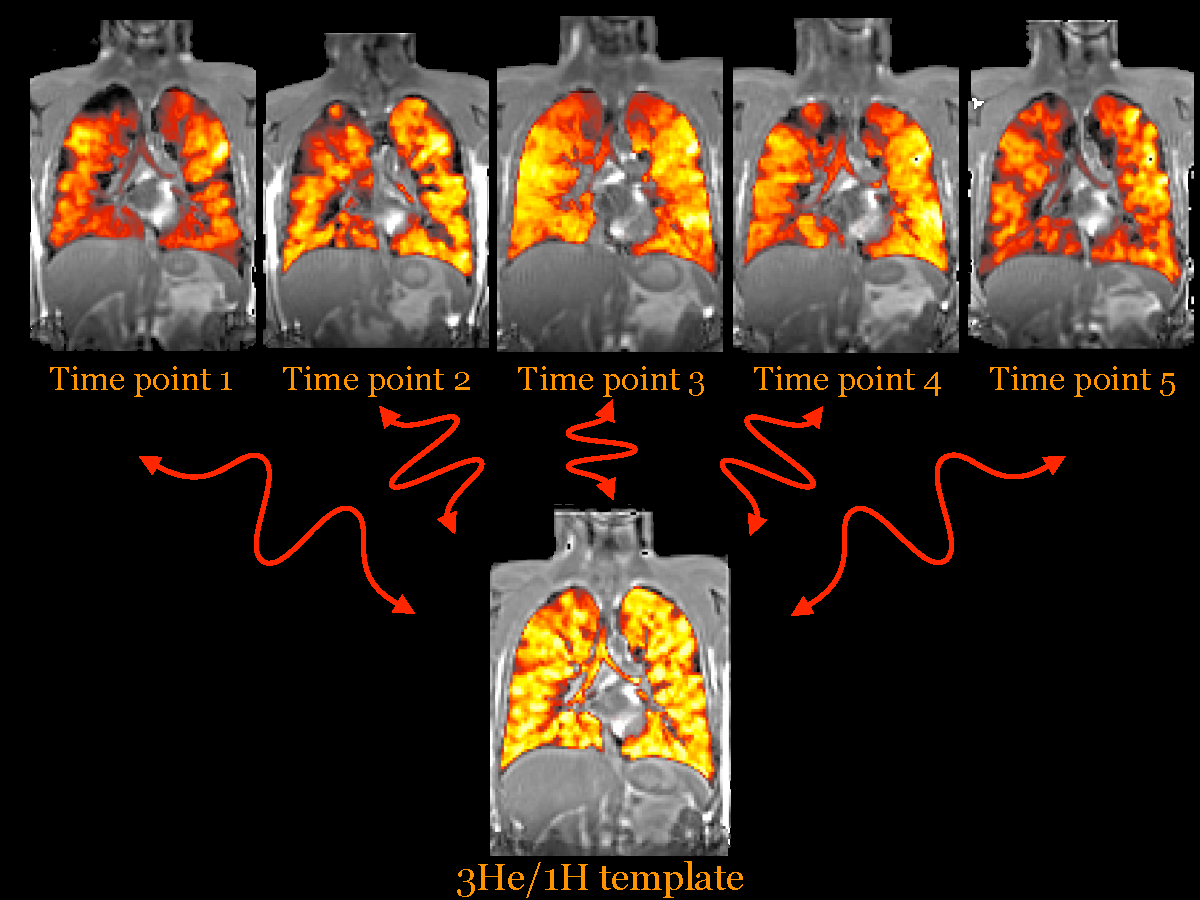
\includegraphics[width=100mm]{H1He3Template.pdf}
\end{tabular}
\end{center}
\caption{Multivariate template construction using both 3He and 1H images.  To create a normalized subject-specific space for statistical analysis of the longitudinal data, a template is created from the 3He and 1H data from each of the five time points.   We show the alignment results of the simultaneous acquisition by overlaying the faux-color rendered 3He image over the grayscale 1H image.  The template is generated iteratively where the algorithm alternates between averaging the registered images and then registering each time point to the average image (i.e. template estimate).}
\label{fig:template}
\end{figure}

In order to perform voxelwise analysis on the longitudinal CF data described previously, we spatially normalize the 3He images to a common reference space (also known as a �template� or �atlas�).  Although resources (both template construction algorithms and pre-constructed templates) are common in the neuroimaging community, they are less well-known in the pulmonary research literature.   %For example, one of the earliest and most widely used templates is the Talaraich atlas created by Dr. Jean Talairach (a French neurosurgeon) who identified landmarks on the post-mortem histological sections of a 60-year old French woman to define a universal, stereotactic cerebral space.  %The utility of a standardized anatomical coordinate system has prompted additional work such as the publicly available Montreal Neurological Institute brain template (Collins, Neelin et al. 1994) which is an average of hundreds of adult brain MRI all registered to the Talaraich atlas.
For the analysis in this work we generate subject-specific templates directly from the image data.  Given the variability in lung shape across populations and the lack of publicly available lung atlases, generating population- or subject-specific templates enhances the accuracy of various analyses including that which is reported in this work.   Applicable to pulmonary data is the template construction algorithm\cite{avants2010} applied to T1-weighted brain data.   However, the simultaneous acquisition of the 3He and 1H images lends itself to multimodal processing in which both modalities are used to simultaneously produce 3He and 1H templates.   This process is represented in Fig. \ref{fig:template} for a single subject. 

Using the simultaneously acquired 3He and 1H data\cite{altes2012} for each of the five time points as input, generation of the subject-specific template(s) can be intuitively understood as iterating between averaging the current set of aligned images to create an estimate of the template and then registering the images to that template estimate (and then repeating for a given number iterations).  More technically, the SyN (Symmetric Normalization) pairwise registration algorithm\cite{avants2011} and an optimized Laplacian sharpening/averaging of the template estimate forms the core of what is denoted as the Symmetric Group Normalization (SyGN) algorithm\cite{avants2010} for template construction.   Given the set of five time point 1H/3He aligned image pairs from a single subject, denoted as $\left\{I_1^{\mathrm{1H}}, I_1^{\mathrm{3He}},\ldots,I_5^{\mathrm{1H}}, I_5^{\mathrm{3He}}\right\}$, template generation involves finding
the set of paired diffeomorphic transformations $\left\{\left(\phi_1,\phi_1^{-1}\right), \ldots,  \left(\phi_5,\phi_5^{-1}\right) \right\}$;
the optimal multimodal template appearance, $J^\mathrm{1H}$ and $J^\mathrm{3He}$; and 
the corresponding coordinate system (i.e. template), $\psi(\mathbf{x})$,
which minimize the cost function
\begin{align}
  \sum_{m=1}^5 \left[
  D\left(\psi(\mathbf{x},\phi_1^m(x,1)\right) + 
  \Pi_{1}\left(I_m^\mathrm{1H}\left(\phi_2^m (\mathbf{x},0.5) \right),J^\mathrm{1H}\left(\phi_1^m (\mathbf{x},0.5) \right)\right) +     
  \Pi_{2}\left(I_m^\mathrm{3He}\left(\phi_2^m (\mathbf{x},0.5) \right),J^\mathrm{3He}\left(\phi_1^m (\mathbf{x},0.5) \right)\right)   \right]
\end{align}
where $D$ is the diffeomorphic shape distance, $D\left( \phi(\mathbf{x},t_a), \phi(\mathbf{x},t_b) \right) = \int_{t_a}^{t_b} \|v(\mathbf{x},t\|_{L}dt$
dependent on the choice of linear operator, $L$, and $v$ is the velocity field, $v\left( \phi(\mathbf{x},t) \right) = \frac{d\phi(\mathbf{x},t)}{dt},\,\, \phi(\mathbf{x},0)=\mathbf{x}$.
Applied to each subject, atlas generation produced subject-specific 1H and 3He template images which constitute a mean shape/appearance model of the image data for all 5 time points.  In addition, each time point image was spatially normalized to the template space in preparation for longitudinal ventilated-based segmentation and subsequent statistical analysis as detailed below.

\subsubsection{Longitudinal ventilation-based segmentation}

Following template construction, preprocessing includes suppression of inhomogeneity artifacts through the application of N4 bias correction\cite{tustison2010} to each individual image.  This step is followed by intensity normalization\cite{nyul2000} where 
the intensities of all 5 time point images are normalized to a single intensity range (only 5 match points were employed to avoid excessive intensity distortion).  Following intensity correction and normalization, the image volumes from each time point are collated into a single spatio-temporal image which is then segmented into four ventilation classes using the Atropos segmentation tool.\cite{tustison2011}  

\subsection{Statistical Processing}

The probabilistic formulation of the Atropos segmentation yields, in addition to the 4-class hard segmentation, a set of four posterior probability maps indicating the maximum a posteriori estimate for each class at each voxel.  These MAP estimates are used to rescale all images to a standard scale denoted as ``expected ventilation'' images.   These rescaled expected ventilation (ev) images are calculated at each voxel, $i$, as follows:
\begin{align}
ev_i = \sum_{l=1}^L l \times \mathrm{Pr}(l|I_i)
\end{align}
where $L$ is the total number of labels (as described above, we use the label set $l \in \{1,2,3,4\}$ to describe the
ventilation classes) and $\mathrm{Pr}(l|I_i)$ is the posterior probability at voxel $i$ (i.e. the probability that voxel $i$ has label $l$ given its intensity value $I$).  The derived expected ventilation maps are then smoothed to reduce slight misalignments.  Voxelwise expected ventilation values are then correlated with the simplified treatment hypothesis (each subject is administered a series of placebos and actual treatments which are hypothesized to result in improved ventilation according to the blue dashed line on the right in Fig. \ref{fig:corr}).  

\begin{figure}
\begin{center}
\begin{tabular}{c}
  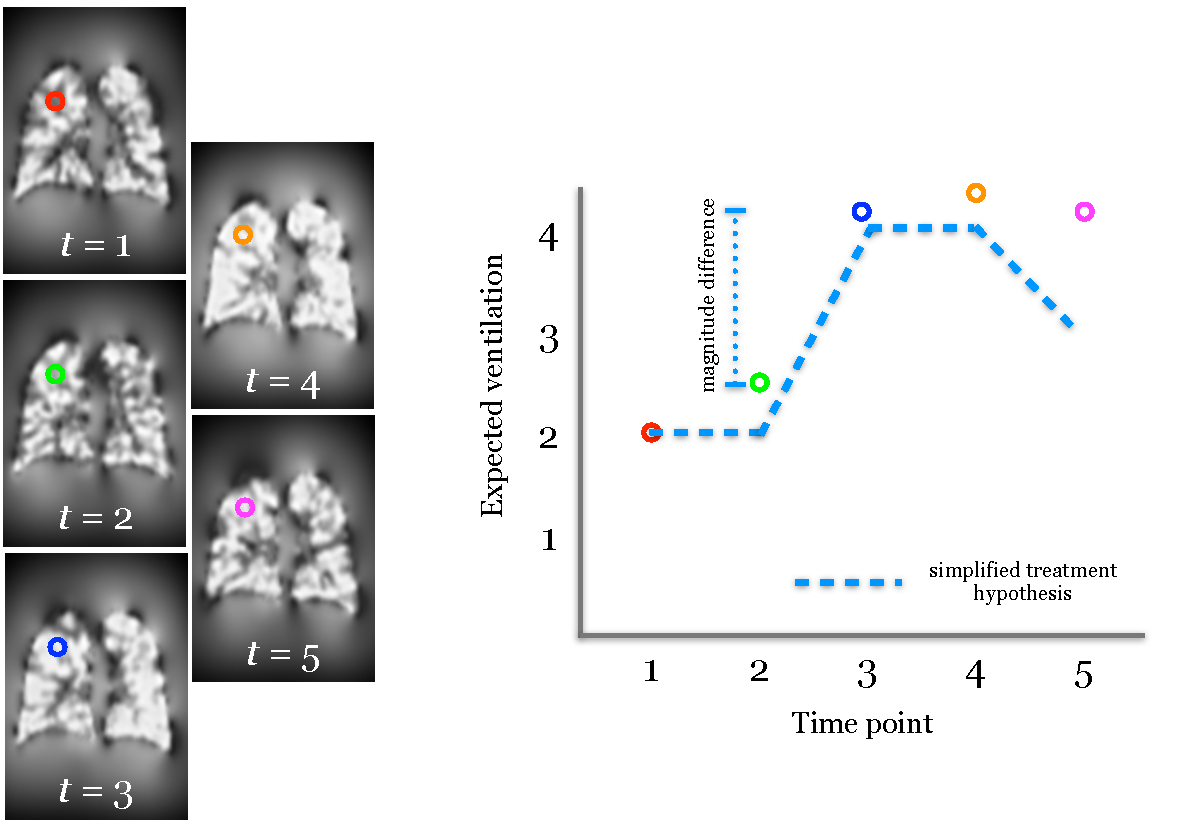
\includegraphics[width=100mm]{correlation.pdf}\\
\end{tabular}
\end{center}
\caption{Voxelwise regression analysis to determine image-based response to treatment.  Treatment effects are expected to follow the simplified treatment hypothesis illustrated with the dashed blue line in the plot on the right.  To explore how the longitudinal change in expected ventilation follows this treatment hypothesis with image data, we smooth the aligned expected ventilation maps (to account for potential voxelwise misalignments) and then quantify how the voxelwise intensities regress with the simplified treatment hypothesis. }
\label{fig:corr}
\end{figure}



%%%%%%%%%%%%%%%%%%%%%%%%%%%%%%%%%%%%%%%%%%%%%%%%%%%%%%%%%%%%%
\section{RESULTS} 

\begin{figure}
\begin{center}
\begin{tabular}{c}
  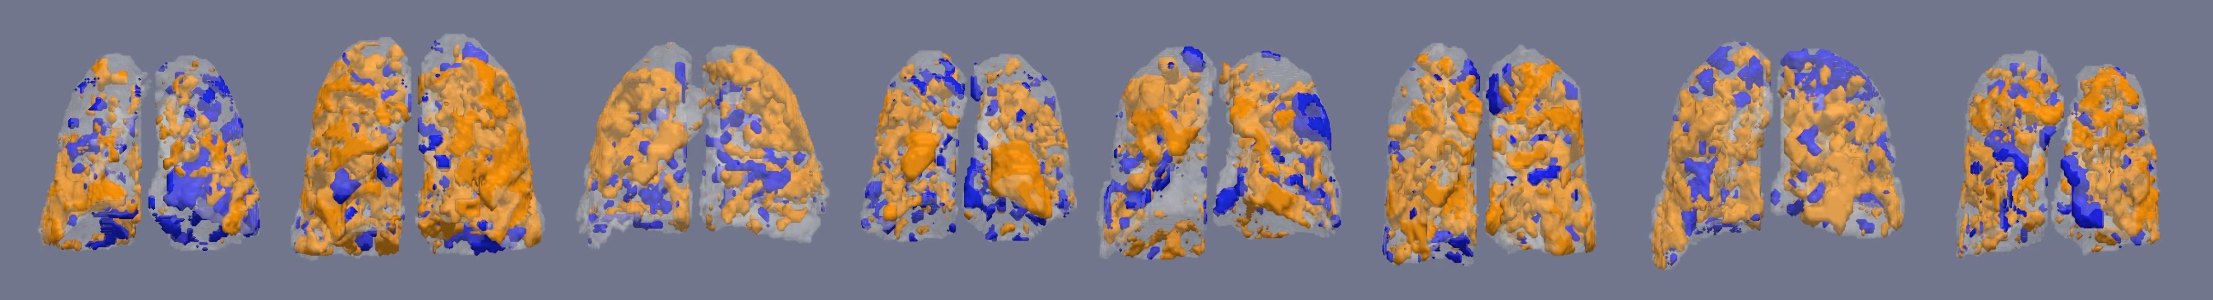
\includegraphics[width=170mm]{3Drenderings.pdf}\\
\end{tabular}
\end{center}
\caption{Resulting signed magnitude maps for all eight subjects showing 
regions of significant positive (orange) and negative (blue) correlations
(where $|$correlation$|$ $\geq 0.50$ and $|ev_{day3} - ev_{day2}| \geq 1.0$) with expected treatment hypothesis.  
}
\label{fig:maps}
\end{figure}

The previously described analysis protocol was applied to each of the eight subjects
to determine spatial response to treatment and subsequently rendered in Fig. \ref{fig:maps}.
Regions of positive correlation (i.e. regions which responded positively to treatment as 
expected) are shown in orange whereas regions of negative correlation (i.e. regions
which became less ventilated during actual treatment) are rendered in blue.  The absolute
correlation threshold of these regions was 0.5.  Additionally, only those regions which 
demonstrated a magnitude expected ventilation value $\geq 1.0$ between days 2 and 3
were rendered.


%%%%%%%%%%%%%%%%%%%%%%%%%%%%%%%%%%%%%%%%%%%%%%%%%%%%%%%%%%%%%
\section{CONCLUSIONS} 
 
Increasing use of imaging for pulmonary longitudinal studies will require computational
techniques for quantifying and visually presenting the data which facilitates
exploration of fundamental clinical hypotheses.  We presented a framework 
for data preparation in single subject longitudinal studies whereby multivariate template
construction results in longitudinal alignment.  This permits such analysis as 
voxelwise statistical regression for determining spatial correlation with expected treatment 
effects.  This provides  a unique visualization technique for exploring clinical
pulmonary hypotheses.


%%%%%%%%%%%%%%%%%%%%%%%%%%%%%%%%%%%%%%%%%%%%%%%%%%%%%%%%%%%%%
%\acknowledgments     %>>>> equivalent to \section*{ACKNOWLEDGMENTS}       
% 
%This unnumbered section is used to identify those who have aided the authors in understanding or accomplishing the work presented and to acknowledge sources of funding.  

%%%%%%%%%%%%%%%%%%%%%%%%%%%%%%%%%%%%%%%%%%%%%%%%%%%%%%%%%%%%%
%%%%% References %%%%%

\bibliography{references}   %>>>> bibliography data in report.bib
\bibliographystyle{spiebib}   %>>>> makes bibtex use spiebib.bst

\end{document} 
